\documentclass[10pt]{article}
 
\usepackage[margin=1in]{geometry} 
\usepackage{amsmath,amsthm,amssymb, graphicx, multicol, array}
\usepackage{enumitem}
\usepackage{hyperref}
\usepackage{multirow}
 
\newcommand{\N}{\mathbb{N}}
\newcommand{\Z}{\mathbb{Z}}
 
\newenvironment{problem}[2][Problem]{\begin{trivlist}
\item[\hskip \labelsep {\bfseries #1}\hskip \labelsep {\bfseries #2.}]}{\end{trivlist}}

\date{Due: Sep 28, 2022 10pm PT}

\begin{document}
 
\title{Assignment 4}
\author{
CS 181AG: Network Algorithmics}
\maketitle

This assignment will give you practice with the Spanning Tree Protocol and Link State Routing. It includes two questions (no programming this week) and a reading assignment with questions.  

\begin{problem} {1: Spanning Tree Protocol}
For the following network, please fill in Rounds 2 and 3 of the table below: for each round, we want to know each bridge's message, its root port, and which other bridges it sends the message to. Similar to in class, assume each connection has a cost of 1, and identify the root port by the bridge at the other end (e.g., B2's root port can be written as ``B1'').

\begin{figure}[h]
    \centering
    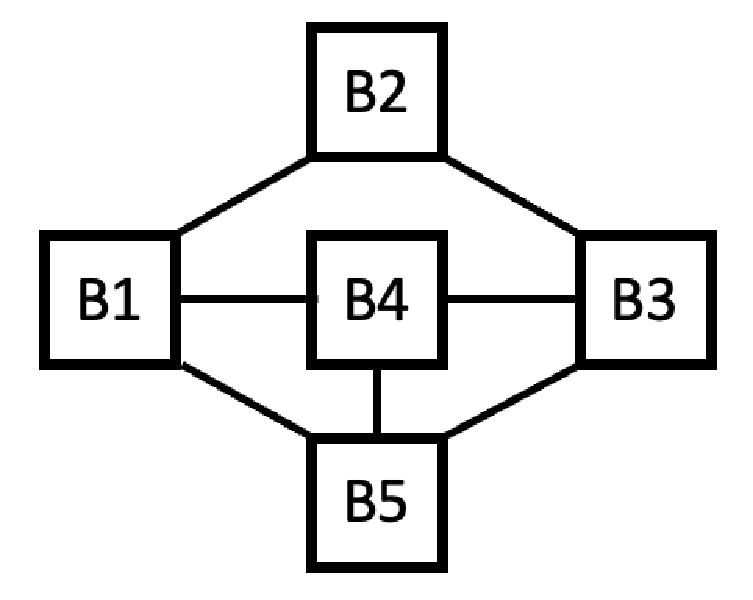
\includegraphics[scale=0.5]{figures/stp.pdf}
    \label{fig:dvp}
\end{figure}

\begin{table}[ht]
\begin{center}
\begin{tabular}{|p{1.2cm}|p{2cm}|p{2.2cm}|p{2.2cm}|p{2.2cm}|p{2.2cm}|p{2.2cm}|}
	\hline
	& & B1 & B2 & B3 & B4 & B5\\
	\hline
	\multirow{6}{*}{Round 1}&Message:  & (B1, B1, 0)& (B2, B2, 0) & (B3, B3, 0) & (B4, B4, 0) & (B5, B5, 0)\\
	& & & & & &\\
	& Root Port: & -& -& -& -& -\\
	& & & & & &\\
	& Sent to: & B2, B4, B5& B1, B3& B2, B4, B5& B1, B3, B5& B1, B3, B4\\
	& & & & & &\\
	\hline
    \multirow{3}{*}{Round 2}&Message: & (B1, B1, 0)& (B2, B1, 1) & (B3, B2, 1) & (B4, B1, 1) & (B5, B1, 1)\\
	& & & & & &\\
	& Root Port: & B1 & B1 & B2 & B1 & B1\\
	& & & & & &\\
	& Sent to: & B2, B4, B5 & B3 & B4, B5 & B3, B5 & B3, B4\\
	& & & & & &\\
	\hline
    \multirow{3}{*}{Round 3}&Message: & (B1, B1, 0) & (B2, B1, 1) & (B3, B1, 2) & (B4, B1, 1) & (B5, B1, 1)\\
	& & & & & &\\
	& Root Port: & B1& B1 & B1 & B1 & B1\\
	& & & & & &\\
	& Sent to: & B2, B4, B5 & B3 & - & B3, B5 & B3\\
	& & & & & &\\
	\hline
    
\end{tabular}
\end{center}
\label{tab:multicol}
\end{table}
\end{problem}

\begin{problem}{2: Link State Routing}
Consider the following graph and assume that each node has successfully sent its local topology to every other node, i.e., each node has a correct and full view of the topology. 

\begin{enumerate}
    \item 
Complete the table below for node u to use Dijkstra's algorithm to calculate its shortest path to each other node. Remember that N is the set of nodes for which we definitively know the shortest path from u, and Q is the set of nodes for which we do not. The first step is completed for you. Note: for each slot in the table, please write the estimated cost and the predecessor, i.e., the node right before the destination in the path, similar to what we did in class. Also, similar to class, leave the spots that correspond to nodes that are already in N blank. Finally, ties in cost can be broken arbitrarily.

\begin{figure}[h]
    \centering
    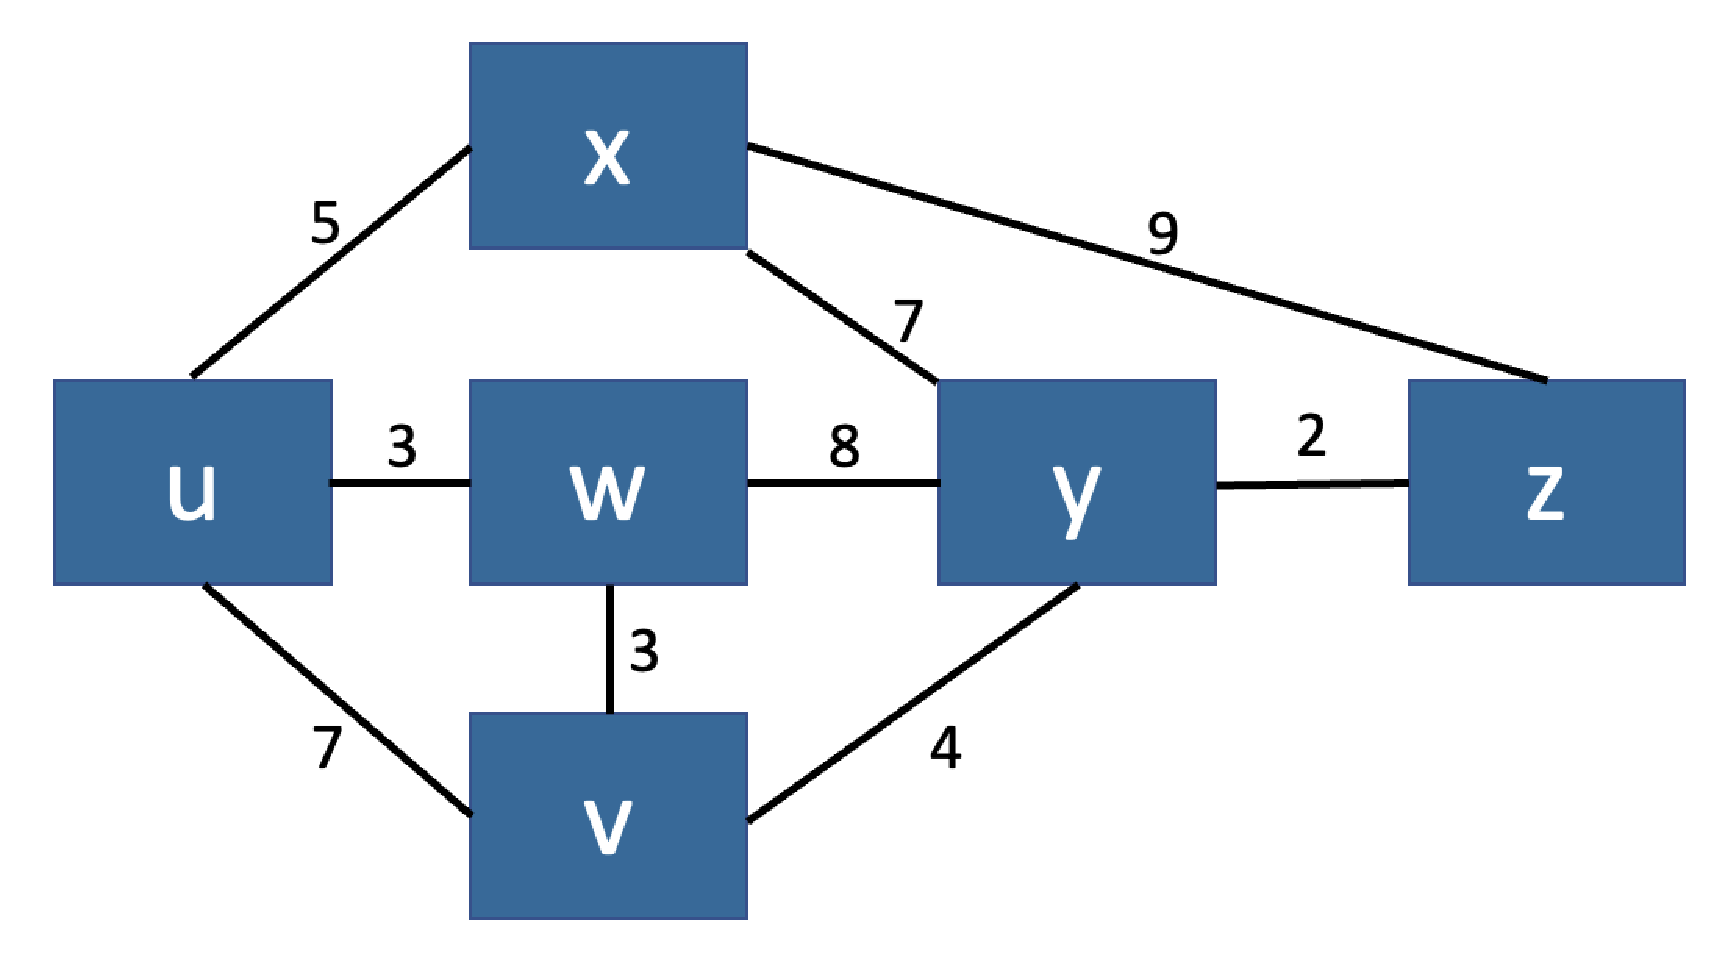
\includegraphics[scale=0.3]{figures/linkstate.pdf}
    \label{fig:dvp}
\end{figure}

\begin{table}[ht]
\begin{center}
\begin{tabular}{|p{1.5cm}|p{1.5cm}|p{1.5cm}|p{1cm}|p{1cm}|p{1cm}|p{1cm}|p{1cm}|}
	\hline
	Step & N & Q & v & w & x & y & z\\
	\hline
	0 & \{u\} & \{vwxyz\} & 7, u& 3, u& 5, u& &\\
	\hline
    1 & \{uw\} & \{vxyz\} &6, w &  & 5, u & 11, w & 14, z\\
	\hline
    2 & \{uwx\} & \{vyz\} & 6, w & & & 11, w & 13, w\\
	\hline
	3 & \{uvwx\}& \{yz\} &  & & & 11, w& 13, w\\
	\hline
	4 & \{uvwxy\} & \{z\} & & & & & 13, w\\
	\hline
	5 & \{uvwxyz\}& & & & & &\\
	\hline
	
\end{tabular}
\end{center}
\label{tab:multicol}
\end{table}
\item Consider the case where the link between w and v breaks. w knows about this broken link immediately and recalculates its shortest paths. Assume that w starts sending according to its new routing table at time t=\emph{a}. u learns about the broken link a short while later, recalculates its shortest paths, and starts sending according to its new routing table at time t=\emph{b}. During the time between \emph{a} and \emph{b}, does data sent from u to v reach successfully? Why or why not?

\item What would be the problem if all routing on the internet was done using link state routing?
\end{enumerate}
\end{problem}

\subsection*{Answer}
\begin{enumerate}
	\item[2.] During the time between $a$ and $b$, we have a termporary loop in which the data sent from u to v does not reach v successfully, since u will try to go through w and v's broken link, but w will try to go through u since it is the cheapest.
	\item[3.] The problem if all routing on the internet was done using link state routing would be the fact that the process does not scale well since each node has to store the full topology of the network. Thus, if it were used for the full internet, then each node would have to store the full toplogy of the internt (all the links as well as then billions of nodes) which takes up a significant amount of space. 
\end{enumerate}

\begin{problem}{3: Reading}
On the course webpage under Assignment 4 - Additional Resources, you'll find a small introduction to vehicle networking. Read this and answer the following questions. Points are for effort.

\begin{enumerate}
    \item What are some of the the main goals of building vehicle networks? 
    \item Write two questions you are curious about after reading this article. 
\end{enumerate}

\subsection*{Answer}
\begin{enumerate}
	\item Some of the main goals of building vehicle networks are highlighted in the "IoVs Distinguishing Characteristics" section of the paper, which include high mobility (since the things are vehicles and are constantly moving around), safety critical applications (the information that is being communicated between vehicles on the network needs to be communicated accurately as well as quickly in order to prevent collisions), vehicle-to-vehicle communciation in a wireless, short-range environment that meets the other criteria since it is infeasible for vicles to be tethered to one another. Some other goals are that the network is secured from malicious agents who may attempt to make up fake data that could have life threatening consequences and that driver behavior and vehicle data should be "privately crowdsourced" meaning that it should not be tied to closely to an individual.
	\item \begin{enumerate}
		\item Is there a particular threshold of number of vehicles for the network to be realistic from both a network support standpoint as well as a number of autonomous cars vs. human drivers standpoint?
		\item What sorts of protocols would be implemented in order to deal with the breaking of links between the different vehicles, such as if there is a network drop or anything along those lines?
	\end{enumerate}
\end{enumerate}

\end{problem}
\begin{problem}{4}
How long did this assignment take you?
\end{problem}
This assignment took me around $\approx 4$ hours.
\end{document}